\documentclass[12pt]{article}
\usepackage{packages}

\addbibresource{bibliography.bib}

\title{\vspace{-2.5em}Calculating the International Geomagnetic Reference Field}
\author{Björn Sundin}

\begin{document}

\maketitle

\section{Introduction}
The International Geomagnetic Reference Field (IGRF) is a three-dimensional model of Earth's internally generated magnetic field that is developed by the International Association of Geomagnetism and Aeronomy (IAGA) \parencite{Alken2021}. A new version is released every five years, because the process by which Earth's magnetic field is generated (magnetohydrodynamic dynamo) causes Earth's magnetic field to change over time.

In a region of space without currents or electromagnetic waves, the Ampère-Maxwell equation becomes $\nabla\crossproduct\vect{B} = 0$ and the field can be written as the negative gradient of a potential $V$; $\vect{B} = -\nabla V$. The IGRF model provides a list of spherical harmonic coeffients $g_n^m$ and $h_n^m$ which are used in the following equation to calculate the potential:
\begin{equation}
  V(r, \theta, \phi) = \sum_{n\,=\,0}^N\frac{a^{n+2}}{r^{n+1}}\sum_{m\,=\,0}^n\left(g_n^m\cos(m\phi) + h_n^m\sin(m\phi)\right)P_n^m(\cos\theta).
\end{equation}
Here $P_n^m(x)$ is the \textit{Schmidt semi-normalized associated Legendre function} of $n$th degree and $m$th order, $a = \SI{6371.2}{\km}$ is Earth's mean radius, $r$ is the distance from Earth's center to the point the magnetic field is to be calculated at, $\theta$ is its co-latitude, and $\phi$ is its longitude. The coefficients are in reality functions of time. The IGRF provides them at five-year intervals, and between these points they can be estimated via linear interpolation. 

Since we are using spherical coordinates, the magnetic field has the form 
\begin{equation}
  \vect{B} = -\nabla V = -\derivative{V}{r}\uvect{r} -\frac{1}{r}\derivative{V}{\theta}\uvect{\theta} - \frac{1}{r\sin\theta}\derivative{V}{\phi}\uvect{\phi}
\end{equation}
and the components can be expanded as
\begin{align}
  B_r &= \sum_{n\,=\,0}^N(n+1)\left(\frac{a}{r}\right)^{n+2}\sum_{m\,=\,0}^n\left(g_n^m\cos(m\phi) + h_n^m\sin(m\phi)\right)P_n^m(\cos\theta)\\ 
  B_\theta &= -\sum_{n\,=\,0}^N\left(\frac{a}{r}\right)^{n+2}\sum_{m\,=\,0}^n\left(g_n^m\cos(m\phi) + h_n^m\sin(m\phi)\right)\derivative{\theta}P_n^m(\cos\theta)\\ 
  B_\phi &= \sum_{n\,=\,0}^N\left(\frac{a}{r}\right)^{n+2}\sum_{m\,=\,0}^n\left(g_n^mm\sin(m\phi) - h_n^mm\cos(m\phi)\right)P_n^m(\cos\theta)
\end{align}
Here we see that we not only need $P_n^m(\cos\theta)$, we also need its derivative with respect to $\theta$.

\section{Associated legendre functions}

The $n$th degree, $m$th order associated legendre function with Schmidt semi-normalization is defined as \parencite{Winch2005}
\begin{equation}
  P_n^m(x) = \alpha_n^m(x)D^{m+n}(x^2-1)^n
\end{equation}
where
\begin{equation}\label{eq:alpha}
  \alpha_n^m(x) = \sqrt{(2-\delta_{m0})\frac{(n-m)!}{(n+m)!}}\frac{1}{2^nn!}(1-x^2)^{m/2},
\end{equation}
$\delta_{m0}$ is the Kronecker delta ($1$ for $m=0$ and $0$ otherwise) and $D = \derivative*{x}$ is the differentiation operator with respect to $x$.

\subsection{Expanded form}
The definition given above involves repeated differentiation, which is not very efficient to implement directly on a computer. The function $Q_n^m(x)=P_n^m(x)/\alpha_n^m(x)$ can be written as a polynomial by first expanding the binomial power:
\begin{equation}
  (x^2 - 1)^n = \displaystyle\sum_{k\,=\,0}^{n}{n\choose k}(-1)^{n-k}x^{2k}
\end{equation}
and then utilizing the following formula for repeated differentiation of a power function
\begin{equation}
  D^{n+m}x^{2k} = \begin{dcases}
    \frac{(2k)!}{(2k-n-m)!}x^{2k-n-m}, &\text{ if }m + n \leq 2k\\
    0, &\text{ if }m + n > 2k
  \end{dcases}.
\end{equation}
Both of these formulas can be proven by induction. Applying them, we get 
\begin{equation}
  Q_n^m(x) = D^{n+m}(x^2 - 1)^2 = \sum_{k\,=\,0}^{n}{n\choose k}(-1)^{n-k}\begin{dcases}
    \frac{(2k)!}{(2k-n-m)!}x^{2k-n-m}, &\text{ if }m + n \leq 2k\\
    0, &\text{ if }m + n > 2k
  \end{dcases}.
\end{equation}
Since
\begin{equation}
  m + n > 2k \iff k < \frac{m+n}{2},
\end{equation}
all terms with $k<\ceil{(m+n)/2}$ are zero, and the equation can be simplified to
\begin{equation}
  Q_n^m(x) = \sum_{k\,=\,\ceil{(m+n)/2}}^{n}{n\choose k}\frac{(2k)!}{(2k-n-m)!}(-1)^{n-k}x^{2k-n-m}.
\end{equation}
This is more readily calculated, although it is still very computationally expensive, with a sum of multiple terms and five factorials to calculate per term. Something we can deduce though is that $Q_n^m(x)=0$ whenever $m+n>2n$, i.e. $m > n$. A faster way to calculate the $Q_n^m$s is to use recurrence relations, and the fact that $Q_n^m(x)=0$ for $m>n$ turns out to be important for doing that.

\subsection{Recurrence relations}
\begin{figure}[htbp]
  \centering
  \begin{tikzpicture}[>=stealth]
    \tikzmath{\nmax= 5;}

    \foreach \n in {0, ..., \nmax} {
      \foreach \m in {0, ..., \n} {
        \node (P\n\m) at (\m, -\n) {$P_{\n}^{\m}$};
      }
    }

    \pgfmathtruncatemacro{\Nminusone}{\nmax-1}
    \foreach \m in {0, ..., \Nminusone} {
      \foreach \n in {\m, ..., \Nminusone} {
        \pgfmathtruncatemacro{\next}{\n+1}
        \draw[->] (P\n\m) -- (P\next\m);
      }
    }

    \foreach \n in {0, ..., \Nminusone} {
      \pgfmathtruncatemacro{\next}{\n+1}
      \draw[->] (P\n\n) -- (P\next\next);
    }
  \end{tikzpicture}
  \caption{Diagram showing how the recurrence relations are used to calculate $P_n^m$.}
  \label{fig:recurrence-diagram}
\end{figure}

Instead of calculating each associated Legendre function by itself, a better idea is to calculate each $P_n^m$ from previously calculated $P_n^m$ values. This is especially fitting for the purposes of calculating the IGRF because we need to use every single $P_n^m$ up to $n=13$, so we are effectively spreading the calculations out between $P_n^m$s and avoid repeating the same calculations many times. 

The recurrence scheme can be done in many different ways. It turns out that doing it row-by-row (where each $n$ is a row and each $m$ is a column) leads to recurrence relations involving division by $\sin\theta$, which leads to the values exploding when near the poles. Instead we do it column-by-column, as illustrated in \autoref{fig:recurrence-diagram}. It all starts from $P_0^0$, which we can calculate to be 
\begin{align}
  P_0^0(x) = \sqrt{(2 - 1)\frac{0!}{0!}}\frac{1}{2^0\cdot 0!}(1 - x^2)^0 = 1
\end{align}
with a derivative with respect to $x$ (or $\theta$, when $x=\cos\theta$) that is identically zero.

The recurrence relations are derived below and are illustrated individually in \autoref{fig:individual-recurrence-relations}; both use two previous values, but one of them might be zero.

\begin{figure}[htbp]
  \centering
  \begin{subfigure}{.25\linewidth}
    \centering
    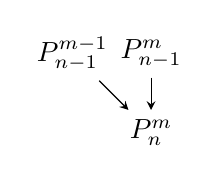
\begin{tikzpicture}[>=stealth]
      \node (Pnm) at (0, 0) {$P_{n}^{m}$};
      \node (Pn1m1) at (-1, 1) {$P_{n-1}^{m-1}$};
      \node (Pn1m) at (0, 1) {$P_{n-1}^{m}$};
      \draw[->] (Pn1m1) -- (Pnm);
      \draw[->] (Pn1m) -- (Pnm);
    \end{tikzpicture}
    \caption{Diagonal}
    \label{fig:recurrence-diag}
  \end{subfigure}
  \begin{subfigure}{.25\linewidth}
    \centering
    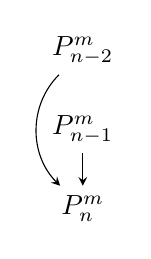
\begin{tikzpicture}[>=stealth]
      \node (Pnm) at (0, 0) {$P_{n}^{m}$};
      \node (Pn1m) at (0, 1) {$P_{n-1}^{m}$};
      \node (Pn2m) at (0, 2) {$P_{n-2}^{m}$};
      \draw[->] (Pn2m) to[out=-135, in=135] (Pnm);
      \draw[->] (Pn1m) -- (Pnm);
    \end{tikzpicture}
    \caption{Downwards}
    \label{fig:recurrence-down}
  \end{subfigure}
  \caption{Diagrams illustrating the two recurrence relations used.}
  \label{fig:individual-recurrence-relations}
\end{figure}

\subsubsection{Diagonal}

The idea for finding the recurrence relations is to use the formula
\begin{equation}
  D^{n}fg = \sum_{k\,=\,0}^{n}{n\choose k}(D^kf)(D^{n-k}g)
\end{equation}
which can also be proven by induction.

Applying it after performing the first derivative, we get
\begin{align}
  Q_n^m &= D^{n+m}(x^2 - 1)^n = D^{n + m - 1}n(x^2 - 1)^{n-1}2x\\ 
  &= 2n\sum_{k\,=\,0}^{n+m-1}{n+m-1\choose k}\left(D^k x\right)\left(D^{n+m-1-k}(x^2 - 1)^{n-1}\right)\\ 
  &= 2n\left(xD^{n+m-1}(x^2 - 1)^{n-1} + (n+m-1)D^{n+m-2}(x^2-1)^{n-1}\right)
\end{align}
and since $Q_{n-1}^{m} = D^{n-1+m}(x^2-1)^{n-1}$ and $Q_{n-1}^{m-1}=D^{n-1+m-1}(x^2-1)^{n-1}$, we get
\begin{equation}\label{eq:recurrence-diag-Q}
  Q_n^m = 2nxQ_{n-1}^m + 2n(n+m-1)Q_{n-1}^{m-1}.
\end{equation}
Since $Q_n^m=P_n^m/\alpha_n^m$, we can rewrite this as 
\begin{equation}
  P_n^m = 2nx\frac{\alpha_n^m}{\alpha_{n-1}^m}P_{n-1}^m + 2n(n+m-1)\frac{\alpha_n^m}{\alpha_{n-1}^{m-1}}P_{n-1}^{m-1}.
\end{equation}
Now we have the recurrence relation illustrated in \autoref{fig:recurrence-diag}. We will want to use this to calculate the topmost values in \autoref{fig:recurrence-diagram}, where $m=n$. But as we saw in the last section, $P_{m-1}^m = 0$. Hence, setting $m = n$ we get 
\begin{equation}\label{eq:recurrence-diag-P-alpha}
  P_m^m = 2m(2m-1)\frac{\alpha_m^m}{\alpha_{m-1}^{m-1}}P_{m-1}^{m-1}.
\end{equation}
Expanding the alphas using equation \eqref{eq:alpha}, we get (assuming $m>0$, since the first value to calculate using this recurrence relation is $P_1^1$)
\begin{align}
  \frac{\alpha_m^m}{\alpha_{m-1}^{m-1}} &= \sqrt{\frac{(2-0)(m-1+m-1)!}{(2-\delta_{m1})(m+m)!}}\frac{1}{2m}\frac{(1-x^2)^{m/2}}{(1-x^2)^{(m-1)/2}}\\ 
                                        &= \sqrt{\frac{1+\delta_{m1}}{2m(2m-1)}}\frac{1}{2m}(1-x^2)^{1/2}
\end{align}
and substituting this back into \eqref{eq:recurrence-diag-P-alpha} results in
\begin{align}
  P_m^m(x) = \sqrt{(1+\delta_{m1})\frac{2m-1}{2m}}(1-x^2)^{1/2}P_{m-1}^{m-1}
\end{align}
or, with $x=\cos\theta$,
\begin{align}
  \boxed{P_m^m(\cos\theta) = \sqrt{(1+\delta_{m1})\left(1-\frac{1}{2m}\right)}\sin(\theta) P_{m-1}^{m-1}(\cos\theta)}
\end{align}

\subsubsection{Downwards}
Finding the recurrence relation shown in \autoref{fig:recurrence-down} was a bit more difficult, and the technique I found involves combining the recurrence relation in \autoref{fig:recurrence-diag} with the one illustrated in \autoref{fig:intermediary-recurrence}.
\begin{figure}[htbp]
  \centering
  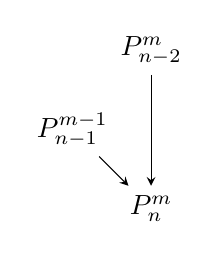
\begin{tikzpicture}[>=stealth]
    \node (Pnm) at (0, 0) {$P_{n}^{m}$};
    % \node[text=gray] (Pn1m) at (0, 1) {$P_{n-1}^{m}$};
    \node (Pn2m) at (0, 2) {$P_{n-2}^{m}$};
    \node (Pn1m1) at (-1, 1) {$P_{n-1}^{m-1}$};
    % \draw[->] (Pn2m) to[out=-45, in=45] (Pnm);
    \draw[->] (Pn2m) -- (Pnm);
    \draw[->] (Pn1m1) -- (Pnm);
  \end{tikzpicture}
  \caption{Recurrence relation used together with the recurrence relation in \autoref{fig:recurrence-diag} to create the downward recurrence relation.}
  \label{fig:intermediary-recurrence}
\end{figure}

This time we start by applying the first two derivatives:
\begin{align}
  Q_n^m &= D^{n+m}(x^2-1)^n = D^{n+m-1}n(x^2-1)^{n-1}2x \\ 
        &= 2nD^{n+m-2}\left((x^2-1)^{n-1}+x(n-1)(x^2-1)^{n-2}2x\right)\\ 
        &= 2nQ_{n-1}^{m-1} + 4n(n-1)D^{n+m-2}x^2(x^2-1)^{n-2}.
\end{align}
Applying the algebraic identity 
\begin{align}
  x^2(x^2-1)^{n-2} = (x^2-1)(x^2-1)^{n-2} + 1(x^2-1)^{n-2} = (x^2-1)^{n-1} + (x^2-1)^{n-2}
\end{align}
and identifying $Q_{n-1}^{m-1}=D^{n+m-2}(x^2-1)^{n-1}$ and $Q_{n-2}^{m}=D^{n+m-2}(x^2-1)^{n-2}$,
\begin{align}
  Q_n^m &= 2nQ_{n-1}^{m-1} + 4n(n-1)\left(Q_{n-1}^{m-1} + Q_{n-2}^m\right)\\ 
        &= 2n(2n - 1)Q_{n-1}^{m-1} + 4n(n-1)Q_{n-2}^m
\end{align}
which corresponds to the diagram in \autoref{fig:intermediary-recurrence}. Now we multiply both sides by $(n+m-1)/(2n-1)$ and rearrange to get 
\begin{align}
  2n(n+m-1)Q_{n-1}^{m-1} = \frac{n+m-1}{2n-1}Q_n^m - \frac{4n(n-1)(n+m-1)}{2n-1}Q_{n-2}^m
\end{align}
which can be substituted in \eqref{eq:recurrence-diag-Q} to give 
\begin{align}
  Q_n^m &= 2nxQ_{n-1}^m + \frac{n+m-1}{2n-1}Q_n^m - \frac{4n(n-1)(n+m-1)}{2n-1}Q_{n-2}^m\\
  \iff \frac{2n-1-n-m+1}{2n-1}Q_n^m &= \frac{n-m}{2n-1}Q_n^m = 2nxQ_{n-1}^m - \frac{4n(n-1)(n+m-1)}{2n-1}Q_{n-2}^m\\ 
  \iff Q_n^m &= \frac{2n(2n-1)}{n-m}xQ_{n-1}^m - \frac{4n(n-1)(n+m-1)}{n-m}Q_{n-2}^m
\end{align}
or 
\begin{align}\label{eq:downward-recurreence-alpha}
  P_n^m = \frac{2n(2n-1)}{n-m}x\frac{\alpha_n^m}{\alpha_{n-1}^m}P_{n-1}^m - \frac{4n(n-1)(n+m-1)}{n-m}\frac{\alpha_n^m}{\alpha_{n-2}^m}P_{n-2}^m.
\end{align}
Using \eqref{eq:alpha} again, the alpha fractions are
\begin{align}
  \frac{\alpha_n^m}{\alpha_{n-1}^m} = \sqrt{\frac{n-m}{n+m}}\frac{1}{2n}
\end{align}
and 
\begin{align}
  \frac{\alpha_n^m}{\alpha_{n-2}^m} = \sqrt{\frac{(n-m)(n-m-1)}{(n+m)(n+m-1)}}\frac{1}{4n(n-1)}.
\end{align}
Back into \eqref{eq:downward-recurreence-alpha}, 
\begin{align}
  P_n^m &= \frac{2n(2n-1)}{n-m}x\sqrt{\frac{n-m}{n+m}}\frac{1}{2n}P_{n-1}^m\\ 
        &- \frac{4n(n-1)(n+m-1)}{n-m}\sqrt{\frac{(n-m)(n-m-1)}{(n+m)(n+m-1)}}\frac{1}{4n(n-1)}P_{n-2}^m. 
\end{align}
After some simplification,
\begin{align}
  \boxed{P_n^m = \frac{2n-1}{\sqrt{n^2-m^2}}xP_{n-1}^m - \sqrt{\frac{(n-1)^2 - 1}{n^2-m^2}}P_{n-2}^m}
\end{align}
% Here we can recognize

% \begin{equation}
%   i = n - m + \begin{cases}
%     \displaystyle\sum_{k\,=\,0}^{m\,-\,1}(N-k), &\text{if }m\neq 0\\
%     0, &\text{if }m=0
%   \end{cases}
% \end{equation}
%
% \begin{equation}
%   \sum_{k\,=\,0}^{m\,-\,1}(N-k) = mN - \sum_{k\,=\,1}^{m\,-\,1}k = mN - \frac{(m-1)m}{2}
% \end{equation}

% \begin{equation}
%   P_n^m(x) = \frac{2n-1}{(n^2 - m^2)^{1/2}}x P_{n-1}^m(x) - \left(\frac{(n-1)^2 - m^2}{n^2 - m^2}\right)^{1/2}P_{n-2}^m(x)
% \end{equation}

\printbibliography

\end{document}
